% !TeX root = RJwrapper.tex
\title{Explaining Predictions with Shapley Values---An Introduction to the
fastshap Package}
\author{by Brandon M. Greenwell}

\maketitle

\abstract{%
An abstract of less than 150 words.
}

\hypertarget{introduction}{%
\subsection{Introduction}\label{introduction}}

Introductory section which may include references in parentheses
\citep{R}, or cite a reference such as \citet{R} in the text.

\hypertarget{background}{%
\subsection{Background}\label{background}}

So what's a Shapley value? The Shapley value is the average marginal
contribution of a \emph{player} across all possible \emph{coalitions} in
a \emph{game}. In the context of statistical/machines learning,

\begin{description}

  \item[Game:] The prediction task for a single observation $x$.
  
  \item[Gain:] The prediction for $x$ minus the average prediction for all training observations.
  
  \item[Players] The feature values of $x$ that collaborate to receive the gain (i.e., predict a certain value).
  
\end{description}

In particular, the Shapley contribution of the \(i\)-th feature to an
instance \(x\) is defined as \begin{equation}
\nonumber
\phi_i\left(x\right) = \frac{1}{p!} \sum_{\mathcal{O} \in \pi\left(p\right)} \left[\Delta Pre^i\left(\mathcal{O}\right) \cup \left\{i\right\} - Pre^i\left(\mathcal{O}\right)\right], \quad i = 1, 2, \dots, p,
\end{equation} where \ldots{}

A simple example may help clarify the main ideas.

\hypertarget{fairly-splitting-a-bar-tab}{%
\subsubsection{Fairly splitting a bar
tab}\label{fairly-splitting-a-bar-tab}}

Alex, Brad, and Brandon decide to go out for drinks after work. They
shared a few pitchers of beer, but nobody payed attention to how much
each person drank. What's a fair way to split the tab? Suppose we knew
the follow information, perhaps based on historical data:

\begin{itemize}

  \item If Alex drank alone, he'd only pay \$10.
  
  \item If Brad drank alone, he'd only pay \$20.
  
  \item If Brandon drank alone, he'd only pay \$10.
  
  \item If Alex and Brad drank together, they'd only pay \$25.
  
  \item If Alex and Brandon drank together, they'd only pay \$15.
  
  \item If Brad and Brandon drank together, they'd only pay \$13.
  
  \item If Ales, Brad, and Brandon drank together, they'd only pay \$30.

\end{itemize}

\begin{table}[]
\centering
\begin{tabular}{@{}llll@{}}
\toprule
                      & \multicolumn{3}{l}{Marginal contribution} \\ \midrule
Permutation           & Alex        & Brad         & Brandon      \\ \midrule
Alex, Brad, Brandon   & \$10        & \$15         & \$5          \\ 
Alex, Brandon, Brad   & \$10        & \$15         & \$5          \\
Brad, Alex, Brandon   & \$5         & \$20         & \$5          \\
Brad, Brandon, Alex   & \$10        & \$20         & \$0          \\
Brandon, Alex, Brad   & \$5         & \$15         & \$10         \\
Brandon, Brad, Alex   & \$17        & \$3          & \$10         \\ \midrule
Shapley contribution: & \$9.50      & \$14.67      & \$5.83       \\ \bottomrule
\end{tabular}
\caption{Marginal contribution for each permutation of Alex, Brad, and Brandon (i.e., the order in which they arrive). The Shapley contribution is the average marginal contribution across all permutations. (Notice how each row sums to the total bill of \$30.)}
\end{table}

So the next time the bartender asks how you want to split the tab, whip
out a pencil and do the math!

\hypertarget{estimating-shapley-values-via-monte-carlo-simulation-sampleshap}{%
\subsubsection{Estimating Shapley values via Monte Carlo simulation:
SampleSHAP}\label{estimating-shapley-values-via-monte-carlo-simulation-sampleshap}}

A single estimate of the contribution of \(x_i\) to \(f\left(x\right)\)
is nothing the more than the difference between two predictions, where
each prediction is based on a sort of Frankenstein instance that' are's
constructed by swapping out values between the instance being explained
(\(x\)) and an instance selected at random from the training data. To
help stabilize the results, the procedure is repeated a large number,
say, \(R\), times, and the result averaged together.

\begin{algorithm}
\begin{enumerate}
  \item For $j = 1, 2, \dots, R$:
  \begin{enumerate}
    \item Select a random permutation $\mathcal{O}$ of the sequence $1, 2, \dots, p$.
    \item Select a random instance $w$ from the training instances $\boldsymbol{X}$.
    \item Construct two new instances as follows:
    \begin{itemize}
      \item $b_1 = x$, but all the features in $\mathcal{O}$ that appear after feature $x_i$ get their values swapped with the corresponding values in $w$.
      \item $b_2 = x$, but feature $x_j$, as well as all the features in $\mathcal{O}$ that appear after $x_j$, get their values swapped with the corresponding values in $w$.
    \end{itemize}
    \item $\phi_{ij}\left(x\right) = f\left(b_1\right) - f\left(b_2\right)$.
  \end{enumerate}
  \item $\phi_i\left(x\right) = \sum_{j = 1} ^ R \phi_{ij}\left(x\right) / R$.
\end{enumerate}
\caption{Approximating the $i$-th feature's contribution to $f\left(x\right)$. \label{alg:SampleSHAP}}
\end{algorithm}

If there are \(p\) features and \(m\) instanced to be explained, this
requires \(2 \times R \times p \times m\) predictions (or calls to a
scoring function). In practice, this can be quite computationally
demanding, especially since \(R\) needs to be large enough to produce
good approximations to each \(\phi_i\left(x\right)\). In practice, this
depends on the variance of each feature in the observed training data,
but typically \(R >= 50--100\) will suffice (\textbf{Need reference}).

\hypertarget{special-cases}{%
\subsubsection{Special cases}\label{special-cases}}

The following sections discuss two special cases where exact Shapley
explanations can be computed efficiently: additive linear models, and
shallow trees and tree ensembles.

\hypertarget{linear-models-linearshap}{%
\paragraph{Linear models: LinearSHAP}\label{linear-models-linearshap}}

Cite somewhere \cite{strumbelj-2014-explaining}.

First, lets discuss how a feature's value contributes to a prediction
\(f\left(X\right)\) in a simple (additive) linear model. That is, let's
assume for a moment that \(f\) takes the form \begin{equation}
\nonumber
  f\left(X\right) = \beta_0 + \beta_1 X_1 + \dots + \beta_p X_p
\end{equation}

Recall that the contribution of the \(i\)-th feature to the prediction
\(f\left(X\right)\) is the difference between \(f\left(X\right)\) and
the expected prediction if the \(i\)-th feature's value were not known:
\begin{equation}
\nonumber
\begin{split}
  \phi_i\left(X\right) &= \beta_0 + \dots + \beta_i X_i + \dots + \beta_p X_p \\ &\quad\quad - \left(\beta_0 + \dots + \beta_i \E\left(X_i\right) + \dots + \beta_p X_p\right) \\
  &= \beta_i \left(X_i - \E\left(X_i\right)\right)
\end{split},
\end{equation} where we estimate \(\E\left(X_i\right)\) with the
corresponding sample mean \(\bar{X}_i\). The quantity
\(\phi_i\left(X\right)\) is also referred to as the
\emph{situational importance of $X_i$} \citep{achen-1982-interpreting}.

\hypertarget{tree-based-models-treeshap}{%
\paragraph{Tree-based models:
TreeSHAP}\label{tree-based-models-treeshap}}

TBD.

\hypertarget{shapley-values-in-r}{%
\subsection{Shapley values in R}\label{shapley-values-in-r}}

TBD.

\hypertarget{so-why-fastshap}{%
\subsubsection{So why fastshap?}\label{so-why-fastshap}}

\hypertarget{efficiency}{%
\paragraph{Efficiency}\label{efficiency}}

Like many post-hoc interpretation techniques (e.g., PDPs and ICE
curves), SampleSHAP can be made more efficient by generating all the
data up front, and scoring it only once (or twice, in the case of
SampleSHAP). For example, PDPs and ICE curves can be efficiently
constructed with only a single call to a scoring function by generating
all of the required data up front using a single cross-join operation
(which can be done rather efficiently in SQL or Spark). The scored data
can then be post-processed/aggregated and displayed as either a PDP or
set of ICE curves. An example using Spark with \CRANpkg{sparklyr}
\citet{R-sparklyr} can be found here:
\url{https://github.com/bgreenwell/pdp/issues/97}.

Fortunately, a similar trick can be exploited for SampleSHAP. Whether
explaining a single instance with a large value of Monte Carlo reps
(\(R\)), or explaining a large number of instances, the basic idea is to
generate all the required Frankenstein instances \(b_1\) and \(b_2\)
upfront, and stored in matrices \(\boldsymbol{B}_1\) and
\(\boldsymbol{B}_2\), respectively.

For example, suppose we wanted to estimate the contribution of \(x_i\)
for each of the \(N\) rows of the available training data
\(\boldsymbol{X}\) using a single Monte-Carlo repetition in
Algorithm\textasciitilde{}\ref{alg:SampleSHAP} (i.e.,
\(R = 1\))\footnote{The same idea also extends to explaining new instances.}.
To start, we can generate the \(N\) random instances at once and store
them in an \(N \times p\) matrix \(\boldsymbol{W}\). Rather generating
\(N\) random permutations \(\mathcal{O}\), and constructing \(b_1\) and
\(b_2\) one at a time, the \pkg{fastshap} package uses C++---via
\CRANpkg{Rcpp} \citep{R-Rcpp}---to efficiently generate an
\(N \times p\) logical matrix \(\boldsymbol{\mathcal{O}}\), where
\(\boldsymbol{\mathcal{O}}_{kl} = 1\) if feature \(x_l\) appears before
feature \(x_i\) in the \(k\)-th permutation, and \(0\) otherwise. This
logical matrix can then be used to logically subset \(\boldsymbol{X}\)
and \(\boldsymbol{W}\) to more efficiently construct
\(\boldsymbol{B}_1\) and \(\boldsymbol{B}_2\) in a single swoop. The
matrices (or data frames) can then be each scored once, and the
difference taken, to generate a single replication of
\(\phi_i\left(x\right)\) for each row of \(\boldsymbol{X}\).

Suppose instead we want to estimate the contribution of \(x_i\) for a
single instance \(x\), but using a large value of \(R\) for accuracy. We
could employ the same trick, but in this case \(\boldsymbol{X}\) would
refer to the \(R \times p\) matrix, where each row is a copy of the
instance \(x\).

\pkg{fastshap} also uses efficient exact methods for the special cases
described in Sections\ldots{}

\hypertarget{parallelization}{%
\paragraph{Parallelization}\label{parallelization}}

\pkg{fastshap} is faster at computing Shapley values for a single
feature for a large number of instances (or a large value of \(R\) for a
single instance). But what about a large number of features?
Fortunately, Algorithm\textasciitilde{}\ref{alg:SampleSHAP} can be
trivially parallelized across features, and this is built into
\pkg{fastshap}.

\hypertarget{a-simple-benchmark-comparison}{%
\paragraph{A simple benchmark
comparison}\label{a-simple-benchmark-comparison}}

This section provides a brief example comparing various implementations
of Shapley values using \href{https://www.kaggle.com/c/titanic}{Kaggle's
Titanic: Machine Learning from Disaster competition}. While the true
focus of the competition is to use machine learning to create a model
that predicts which passengers survived the Titanic shipwreck, we'll
focus on explaining predictions from a simple logistic regression model.

To start, we'll load the data, which are conveniently available in the
\CRANpkg{titanic} package \citep{R-titanic}, and do a little bit of
cleaning.

\begin{Schunk}
\begin{Sinput}
# Read in the data and clean it up a bit
titanic <- titanic::titanic_train
features <- c(
  "Survived",  # passenger survival indicator
  "Pclass",    # passenger class
  "Sex",       # gender
  "Age",       # age
  "SibSp",     # number of siblings/spouses aboard
  "Parch",     # number of parents/children aboard
  "Fare",      # passenger fare
  "Embarked"   # port of embarkation
)
titanic <- titanic[, features]
titanic$Survived <- as.factor(titanic$Survived)
titanic <- na.omit(titanic)

# Data frame containing just the features
X <- subset(titanic, select = -Survived)
\end{Sinput}
\end{Schunk}

Next, we'll use the stats::glm() to fit a logistic regression model with
only main effects (i.e., no tw-way interactions, etc.).

\begin{Schunk}
\begin{Sinput}
fit <- glm(Survived ~ ., data = titanic, family = binomial)
\end{Sinput}
\end{Schunk}

Suppose we wanted to explain the predicted survival probability for a
new passenger named Jack:

\begin{Schunk}
\begin{Sinput}
jack <- data.frame(
  Pclass = 3,
  Sex = factor("male", levels = c("female", "male")),
  Age = 20,
  SibSp = 0,
  Parch = 0,
  Fare = 15,  # lower end of third-class ticket prices
  Embarked = factor("S", levels = c("", "C", "Q", "S"))
)
\end{Sinput}
\end{Schunk}

Our logistic regression model predicts that Jack's log-odds of survival
is

\begin{Schunk}
\begin{Sinput}
predict(fit, newdata = jack)
\end{Sinput}
\begin{Soutput}
#>         1 
#> -1.845561
\end{Soutput}
\end{Schunk}

Yikes, that's equivalent to estimated 13.64\% predicted probability of
survival! With a baseline (i.e., average) survival rate of 40.62\%, can
we explain why the model predicts Jack to be much lower?
Enter\ldots Shapley values.

There is a growing number of R packages that provide Shapley
explanations, the two most popular arguably being \pkg{iml} and
\pkg{iBreakDown}. In this example, we'll compare those with
\pkg{fastshap}.

To start, we need to define a few things (prediction wrapper, as well as
both \pkg{iml}- and \pkg{iBreakDown}-related helpers).

\begin{Schunk}
\begin{Sinput}
# Prediction wrapper to compute predicted probability of survive
pfun <- function(object, newdata) {
  predict(object, newdata = newdata)
}

# DALEX-based helper for iBreakDown
explainer <- DALEX::explain(fit, data = X, y = titanic$Survived,                                             predict_function = pfun, verbose = FALSE)

# Helper for iml
predictor <- iml::Predictor$new(fit, data = titanic, y = "Survived",
                                predict.fun = pfun)
\end{Sinput}
\end{Schunk}

Next, we call each implementation's Shapley-related function to compute
explanations for Jack's prediction using 100 Monte Carlo repetitions.

\begin{Schunk}
\begin{Sinput}
# Compute explanations
set.seed(1039)  # for reproducibility
ex1 <- iBreakDown::shap(explainer, B = 100, new_observation = jack)
ex2 <- iml::Shapley$new(predictor, x.interest = jack, sample.size = 100)
ex3 <- fastshap::explain(fit, X = X, pred_wrapper = pfun, nsim = 100,
                         newdata = jack)

# Plot results
library(ggplot2)  # for `autoplot()` function
p3 <- plot(ex1) + ggtitle("iBreakDown")
p2 <- plot(ex2) + ggtitle("iml")
p1 <- autoplot(ex3, type = "contribution") + ggtitle("fastshap")
fastshap::grid.arrange(p1, p2, p3, nrow = 1)
\end{Sinput}
\begin{figure}[!htb]

{\centering 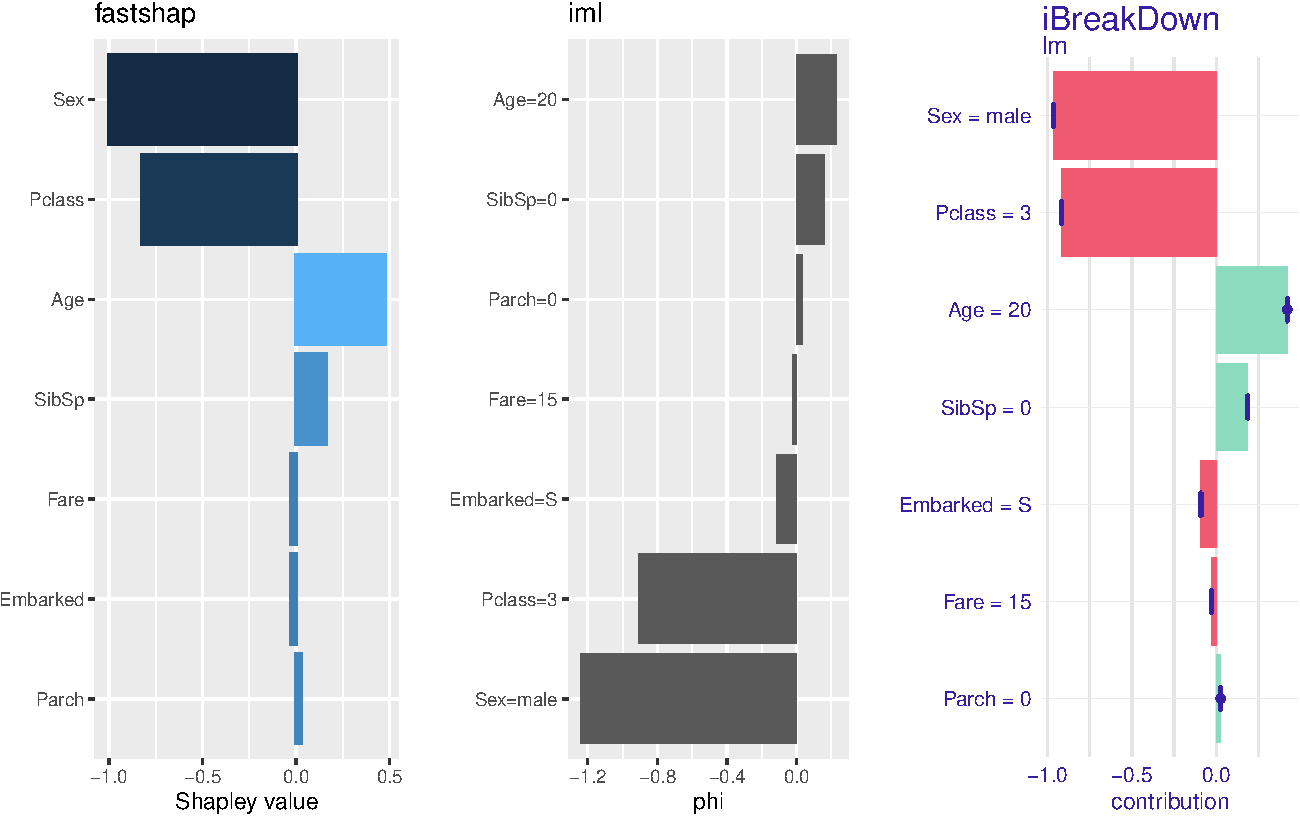
\includegraphics[width=1\linewidth]{greenwell_files/figure-latex/titanic-jack-explanations-1} 

}

\caption[TBD]{TBD.}\label{fig:titanic-jack-explanations}
\end{figure}
\end{Schunk}

Each package comes loaded with it's own bells and whistles (e.g.,
\pkg{iml} and \pkg{iBreakDown} have particularly fantastic
visualizations). The main selling point of \pkg{fastshap} is speed! For
example, all three packages (in fact, all general and practical
implementations of Shapley values) use
Algorithm\textasciitilde{}\ref{alg:SampleSHAP} which requires a large
number of Monte Carlo repetitions to achieve accurate results. Below is
a simple benchmark looking at the estimated time (in seconds) to explain
Jack's prediction as a function of the number of Monte Carlo repetitions
for each implementation. (Note that this comparison does not make use of
\pkg{fastshap}'s feature-wise parallelization.)

\begin{Schunk}
\begin{Sinput}
nsims <- c(1, 5, 10, 25, 50, 75, seq(from = 100, to = 1000, by = 100))
times1 <- times2 <- times3 <- numeric(length(nsims))
set.seed(904)
for (i in seq_along(nsims)) {
  message("nsim = ", nsims[i], "...")
  times1[i] <- system.time({
    iBreakDown::shap(explainer, B = nsims[i], new_observation = jack)
  })["elapsed"]
  times2[i] <- system.time({
    iml::Shapley$new(predictor, x.interest = jack, sample.size = nsims[i])
  })["elapsed"]
  times3[i] <- system.time({
    fastshap::explain(fit, X = X, newdata = jack, pred_wrapper = pfun, 
                      nsim = nsims[i])
  })["elapsed"]
}
pal <- palette.colors(3, palette = "Okabe-Ito")  # colorblind friendly palette 
plot(nsims, times1, type = "b", xlab = "Number of Monte Carlo repetitions",
     ylab = "Time (in seconds)", las = 1, pch = 19, col = pal[1L],
     xlim = c(0, max(nsims)), ylim = c(0, max(times1, times2, times3)))
lines(nsims, times2, type = "b", pch = 19, col = pal[2L],)
lines(nsims, times3, type = "b", pch = 19, col = pal[3L],)
legend("topleft",
       legend = c("iBreakDown", "iml", "fastshap"),
       lty = 1, pch = 19, col = pal, inset = 0.02)
\end{Sinput}
\begin{figure}[!htb]

{\centering 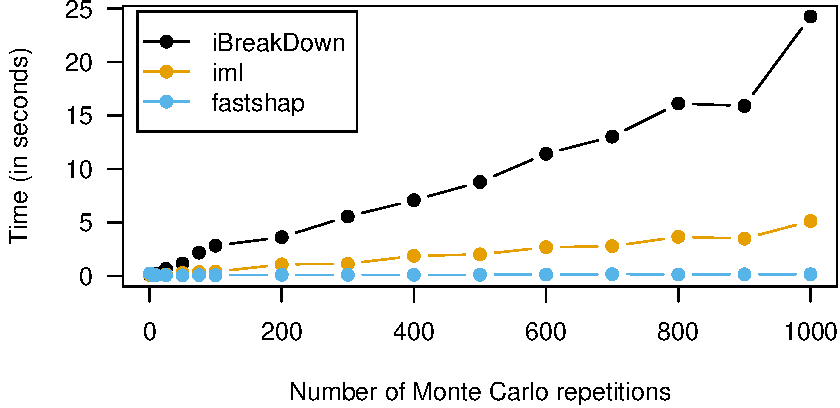
\includegraphics[width=0.8\linewidth]{greenwell_files/figure-latex/titanic-benchmark-1} 

}

\caption[Quick benchmark between three different implementations of SampleSHAP for explaining Jack's unfortunate prediction]{Quick benchmark between three different implementations of SampleSHAP for explaining Jack's unfortunate prediction.}\label{fig:titanic-benchmark}
\end{figure}
\end{Schunk}

The message to be taken from
Figure\textasciitilde{}\ref{fig:titanic-benchmark} is that
\pkg{fastshap} scales incredibly well with \(N\) or \(R\), as long as
the corresponding \code{predict()} method does.

Oh, and \pkg{fastshap} can produce instant (and exact) Shapley
contributions for this example.

\begin{Schunk}
\begin{Sinput}
fastshap::explain(fit, newdata = jack, exact = TRUE)  # ExactSHAP
\end{Sinput}
\begin{Soutput}
#> # A tibble: 1 x 7
#>   Pclass    Sex   Age SibSp  Parch    Fare Embarked
#>    <dbl>  <dbl> <dbl> <dbl>  <dbl>   <dbl>    <dbl>
#> 1 -0.915 -0.964 0.420 0.186 0.0260 -0.0282  -0.0919
\end{Soutput}
\begin{Sinput}
fastshap::explain(fit, X = X, pred_wrapper = pfun, nsim = 10000,
                  newdata = jack)  # SampleSHAP
\end{Sinput}
\begin{Soutput}
#> # A tibble: 1 x 7
#>   Pclass    Sex   Age SibSp  Parch    Fare Embarked
#>    <dbl>  <dbl> <dbl> <dbl>  <dbl>   <dbl>    <dbl>
#> 1 -0.929 -0.977 0.422 0.185 0.0257 -0.0290  -0.0865
\end{Soutput}
\begin{Sinput}
predict(fit, newdata = jack, type = "terms")  # ExactSHAP (base R)
\end{Sinput}
\begin{Soutput}
#>       Pclass        Sex       Age     SibSp      Parch       Fare    Embarked
#> 1 -0.9153946 -0.9644851 0.4204564 0.1861824 0.02599872 -0.0281944 -0.09194646
#> attr(,"constant")
#> [1] -0.4781785
\end{Soutput}
\end{Schunk}

\hypertarget{example-predicing-sales-prices}{%
\subsection{Example: predicing sales
prices}\label{example-predicing-sales-prices}}

TBD.

\hypertarget{example-default-of-credit-card-clients}{%
\subsection{Example: default of credit card
clients}\label{example-default-of-credit-card-clients}}

TBD.

\hypertarget{summary}{%
\subsection{Summary}\label{summary}}

This file is only a basic article template. For full details of
\emph{The R Journal} style and information on how to prepare your
article for submission, see the
\href{https://journal.r-project.org/share/author-guide.pdf}{Instructions
for Authors}.

\bibliography{greenwell}


\address{%
Brandon M. Greenwell\\
University of Cincinnati\\
2925 Campus Green Dr\\ Cincinnati, OH 45221\\ United States of America\\ ORCiD---\href{https://orcid.org/0000-0002-8120-0084}{0000-0002-8120-0084}\\
}
\href{mailto:greenwell.brandon@gmail.com}{\nolinkurl{greenwell.brandon@gmail.com}}

